\documentclass[11pt,letterpaper,notitlepage]{article}

% Codificación GNU/Linux
\usepackage[utf8]{inputenc}
\usepackage[activeacute,spanish]{babel}

% Margenes
\usepackage{anysize}
\marginsize{2cm}{2cm}{2cm}{2cm}

% Simbolos y letras para matemáticas
\usepackage{amssymb,amsmath,amsfonts}

% Colores
\usepackage{xcolor}
\definecolor{rojo}{RGB}{255,26,34}
\definecolor{azul}{RGB}{0,0,250}
\definecolor{gris_oscuro}{RGB}{90,90,90}
\definecolor{gris}{RGB}{210,210,210}

% Elementos Flotantes (Figuras y Tablas)
\usepackage{graphicx}
\usepackage{float}
\usepackage{multicol}
\usepackage{multirow}
\usepackage{subfigure}
\usepackage{epstopdf}
\usepackage{enumerate}
\graphicspath{ {img/} } % Carpeta de imagenes
%------ CONFIGURACIÓN LINKS ---------
\usepackage{hyperref}
\hypersetup{
    colorlinks,
    linkcolor={azul},
    citecolor={azul},
    urlcolor={azul}
}

%------ CÓDIGO ARDUINO ---------
\usepackage{listings}
\def\commentfont{\color[gray]{.5}\itshape}
\def\keywordfont{\color[RGB]{255,100,0}\bfseries}
\lstset{						%
language=c++,					%Lenguaje
basicstyle=\footnotesize\ttfamily,%Tamaño de fuente
numbers=left,					%Donde poner los números de lines
numberstyle=\footnotesize,		%Tamaño de números de linea
stepnumber=1,					%Saltos en números de linea
numbersep=5pt,					%
backgroundcolor=\color{white},	%Color de fondo
showspaces=false,               %Mostrar espacios
showstringspaces=false,         %Subrayar espacios
showtabs=false,                 %Mostrar tabulacion
frame=single,					%Añadir marco
tabsize=2,						%Tamaño del tab
captionpos=b,					% sets the caption-position to bottom
breaklines=true,				% sets automatic line breaking
breakatwhitespace=false,		% sets if automatic breaks should only happen at whitespace
keywordstyle=\keywordfont,		%Palabras clave en amarillo
commentstyle=\commentfont,      %Comentarios en gris
stringstyle=\color[RGB]{0,128,128}	%Strings en celeste
}
\renewcommand{\lstlistingname}{Código fuente}
\renewcommand{\lstlistlistingname}{Índice de códigos fuente}

%Bloque atención
\usepackage[tikz]{bclogo}
\newcommand*\atencion[1]{
   \vspace{0.5cm}
   \begin{bclogo}[couleur=gris, logo=\bcattention, noborder=true]{Atención}
     {#1} 
   \end{bclogo}
   \vspace{3mm}}
   
\newcommand*\info[1]{
   \vspace{0.5cm}
   \begin{bclogo}[couleur=gris, logo=\bcinfo, noborder=true]{Información}
     {#1} 
   \end{bclogo}
   \vspace{3mm}}
   
\newcommand*\correccion[1]{
   \vspace{0.5cm}
   \begin{bclogo}[couleur=gris, logo=\bcoutil, noborder=true]{Correcciones}
     {#1} 
   \end{bclogo}
   \vspace{3mm}}


\begin{document}


\begin{figure}
\vspace*{-1.5cm}
\begin{minipage}[c]{0.5\textwidth}
	
\includegraphics{../img/fcfm}
\end{minipage} \hfill \begin{minipage}[t]{0.4\textwidth}
\begin{flushright}
	EI2001 - Robótica y Mecatrónica \\
	Profesor: Javier Ruiz del Solar \\
	Otoño 2015
\end{flushright}
\end{minipage}
\noindent\makebox[\linewidth]{\rule{\textwidth}{1pt}}
\end{figure}

\begin{center}
\huge Guía Teórica \#1 \\
\Large \textbf{Principios básicos de electrónica}
\end{center}

\section{Introducción}

Esta guía cubre los conceptos básicos de electrónica, como corriente, voltaje, resistencia, potencia y otros más que son importantes para comprender el funcionamiento de circuitos electrónicos. Usando leyes de Kirchoff y la ley de Ohm, se presentarán métodos para analizar circuitos simples compuestos por elementos resistivos.

\section{Corriente}

La corriente eléctrica (simbolizada por \textit{I}) representa la cantidad de carga eléctrica $\Delta Q$ que atraviesa una sección transversal por unidad de tiempo, esta dada por

\begin{equation}
I=\frac{\Delta Q}{\Delta t}
\end{equation}

La unidad de medida para la intensidad de corriente eléctrica es el amperio o \textit{ampere} (\textit{A}). La corriente eléctrica es típicamente un flujo de electrones a través de un conductor, sin embargo, por convención se usa como portador cargas positivas, esto significa que dado un flujo de electrones en una dirección, la corriente \textit{I} se mueve en dirección opuesta, como muestra la figura \ref{corriente}.

\begin{figure}[H]
\begin{center}
	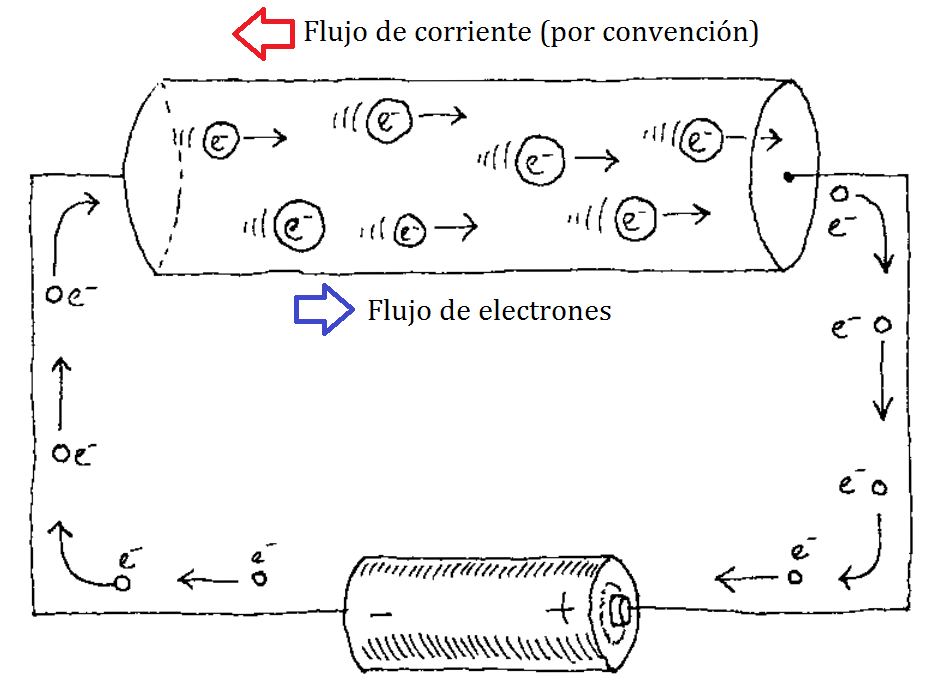
\includegraphics[scale=0.3]{corriente}
	\caption{Convención de corriente.}
	\label{corriente}
\end{center}
\end{figure}

\section{Voltaje}



\end{document}
